\section{Calcium Borohydride [$\beta$-\ce{Ca(BH4)2}]}
\label{sec:borohydrides-calcium}

\bit
\item Prepare HTST rates and compare with experiments
\item Revise the experimental rates as applicable
\item Do further MEP calculations for mechanisms that still remain unexplained in the experimental data
\eit

The calculational parameters can be found in DFT Calculations section of Paper \ref{pap:calcium}.

The experimental data suggested three separate processes, two of which were assigned to rotational diffusion of hydrogen, while the latter was assigned to longer range diffusion of hydrogen.

\subsubsection{Rotation of \ce{BH4-}}
The bulk of the initial data from the QENS experiments indicated rotational diffusion of hydrogen, while possible high temperature long-range diffusion was also detected.
Thus, the work focused mainly on rotations around the possible symmetry axes, $C_2$ and $C_3$, of the \ce{BH4-} unit.
By choosing the appropriate axes, a contour plot of the rigid rotation was produced in order to get an overview of the possible rotations, pure or coupled, and an estimate of their relative barrier heights.

\begin{figure}[h]
\begin{center}
  \subfigure[Potential Energy Surface for \ce{Ca(BH4)2}][Potential Energy Surface for \ce{Ca(BH4)2} with MEPs and the local environment overlayed.]{
    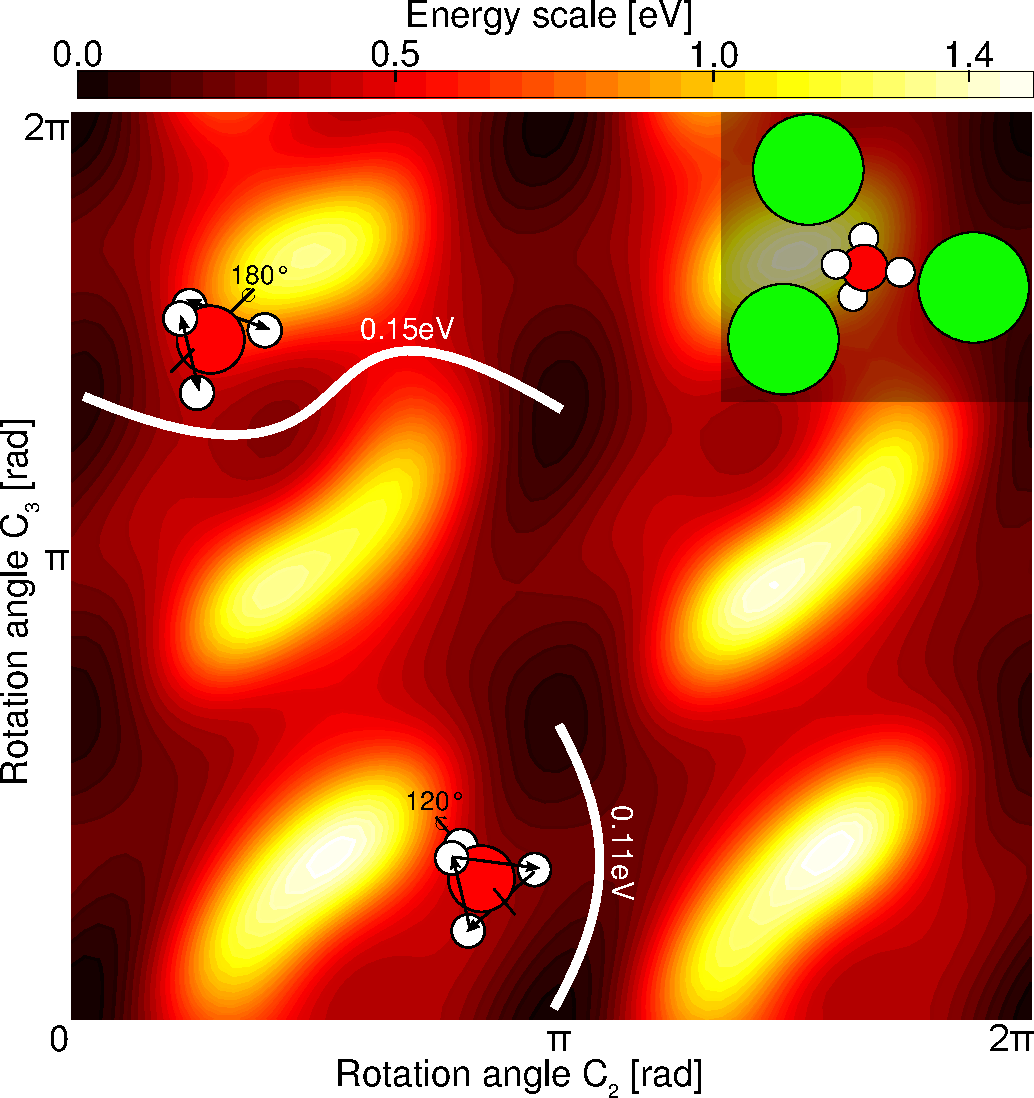
\includegraphics[width=0.35\linewidth]{ca-pes01}
    \label{fig:ca-pes01}
    }
  \subfigure[\ce{Ca(BH4)2} energy profiles][\ce{Ca(BH4)2} energy profiles. The blue circles represent the $C_2$-type rotation and the red squares represent the $C_3$-type rotation.]{
    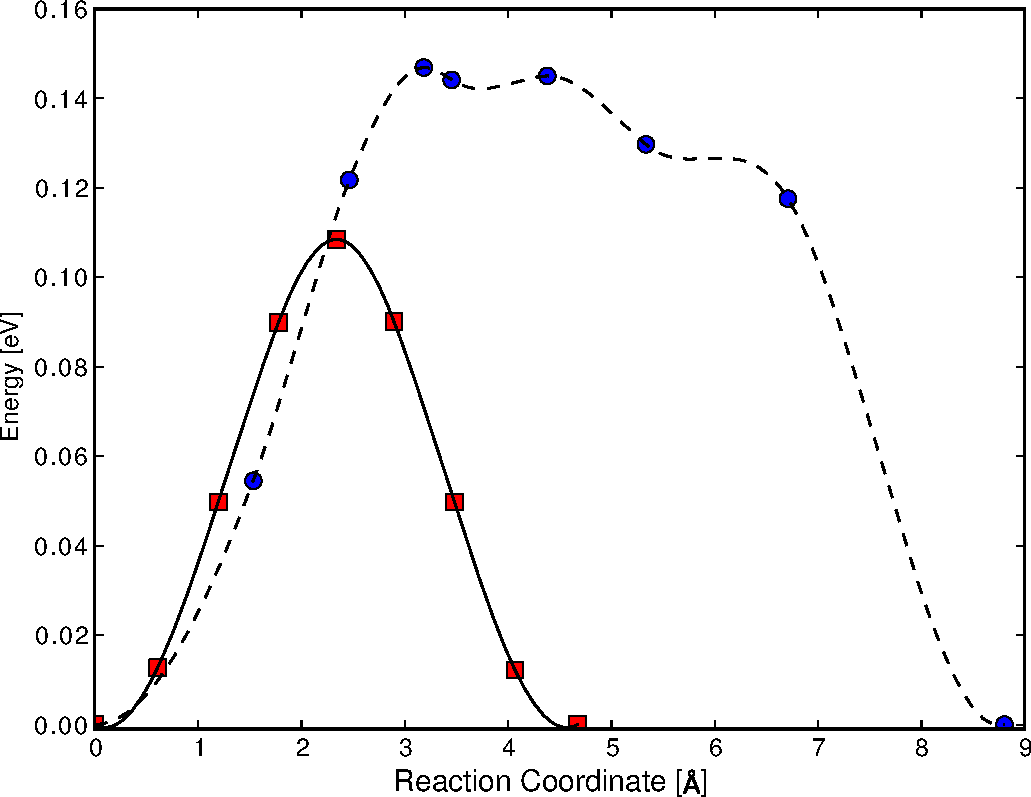
\includegraphics[width=0.45\linewidth]{ca-barriers}
    \label{fig:ca-barriers}
    }
    \parbox{0.85\linewidth}{
      \caption{The rotational analysis of \ce{BH4-} in \ce{Ca(BH4)2}.
      The figures are taken from paper \ref{pap:calcium}
It should be noted that some symmetry breaking can be seen in the PES, which is to be expected as the tetragonal symmetry is slightly broken during the minimisation, due to the environment.
      }
      \label{fig:ca-rotational}
    }
\end{center}
\end{figure}

Since the rotational system has three dimensions but the contourplot has only two, the axes had to be chosen carefully as to sample all interesting events.
Each $C_2$ axis roughly lines up with a \ce{Ca}-\ce{B} vector, which means that with regards to symmetry they are all nearly equivalent.
The one with maximal \ce{H}-\ce{Ca} distance was chosen as one of the contour axes.
The choice of the $C_3$ axis had a similar goal, to minimise \ce{H}-\ce{Ca} interaction.
This was accomplished by choosing the axis which lies closest to the plane spanned by the three nearest neighbor calcium atoms.
This axis samples half of the possible $C_3$ axes when the full $C_2$ rotation is taken into account.
Due to symmetrical similarity it is likely that the remaining $C_3$ axes are indirectly sampled also.

The contour plots give an important insight as to which of the possible rotations are the interesting ones and, thus, calculating the more resource intensive MEPs can be limited to the interesting processes.
\Fref{fig:ca-pes01} shows that a $C_3$ axis is lowest in energy and that a wobbly $C_2$ axis with a small intermediate minimum is the lowest energy $C_2$ type rotation.
Using these as the starting paths for NEB calculations, the MEPs, shown overlayed in \fref{fig:ca-pes01}, are found and shown as energy profiles in \fref{fig:ca-barriers}.

Right away, the theoretical data was in good agreement with the experimental data, nevertheless, further refinement of the experimental data was possible after the theoretical data was complete, which yielded better agreement for the rotational data and an extra point for the possible long range diffusion.
This beautifully illustrates how theory and experiments complement and can be used to benefit each other.

In the end, the calculations complemented the experimental data very well, both with regards to the barrier height as well as the charactristic times which are derived from the HTST reaction rates. (see Table 2 in Paper \ref{pap:calcium})

\subsubsection{Long-range diffusion \pending}
Multiple diffusional species and mechanisms can easily be imagined.
Vacancy mediated \ce{BH3},  \ce{BH4} and \ce{H} diffusion, interstitial hydrogen, atomic and molecular, and two different interstitial waters were all investigated, the results shown in table 3 of paper \ref{pap:calcium}.

The vacancies all had high formation energies, $1.56\unit{eV}$ - $2.83\unit{eV}$, and barriers, $0.46\unit{eV}$ - $1.92\unit{eV}$.
The stable interstital defects, had lower formation energies, $-0.05\unit{eV}$ - $0.40\unit{eV}$, and barriers, $0.09\unit{eV}$ - $0.68\unit{eV}$.
The \ce{H}-interstitial proved to be unstable and formed a \ce{H2}-interstatial coupled to a \ce{H}-vacancy.

The only defect that agreed to any significance with the experimental data, was the \ce{H2}-interstitial.
The characteristic times were not in full agreement though but this might very well be due to the lack of experimental data points, since only two were available for a linear interpolation on an Arrhenius type plot (figure 10 in paper \ref{pap:calcium}).

